\section{Wang Mason}

\begin{frame}
\frametitle{Wang Mason Model \cite{wangmason}}
\begin{itemize}
    \item 2D Impact Model with Friction
    \item Inputs:
    \begin{itemize}
        \item Geometric and mass properties
        \item Pre-impact state
        \item Frictional coefficient ($\mu$)
        \item Coefficient of restitution ($\epsilon$)
    \end{itemize}
\end{itemize}   
\begin{figure}
    \centering
    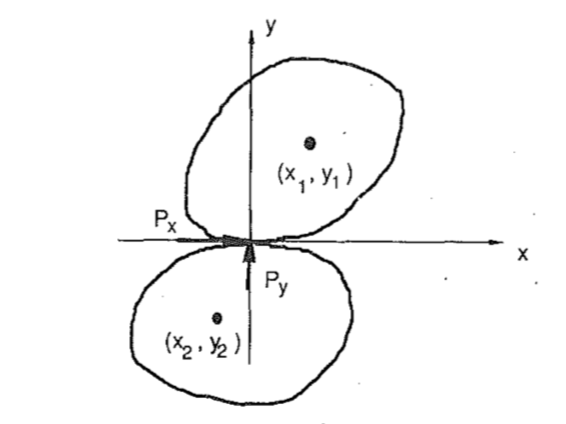
\includegraphics[scale=0.6]{figures/WangPlot.png}
    \caption{Two colliding rigid bodies in a plane\cite{wangmason}}
    \label{fig:WangPlot}
\end{figure}

\end{frame}


\subsection{Implementation}

\begin{frame}{Implementing the Wang Mason Model}
\begin{table}[h!]
    \centering
    \begin{tabular}{|c|c|c|}
        \hline
         & $\mu > |\mu_s|$ & $\mu < |\mu_s|$ \\
         \hline
         $P_d > (1+e)P_q$  & \multicolumn{2}{c|}{Sliding} \\
         \hline
         $P_q < P_d < (1+e)P_q$ & R-Sticking & R-Reversed Sliding \\
         \hline
         $P_d < P_q$ & C-Sticking & C-Reversed Sliding\\
         \hline
    \end{tabular}
    \caption{Analytical Method for Determining Contact Mode}
\end{table}

\begin{itemize}
    \item Each contact mode has their own unique two equations to solve for the impulses ($P_x$ and $P_y$)
    \item From this, we have a function that can take the pre-impact state and some properties from the system and predict a post-impact state
\end{itemize}

\end{frame}

\subsection{Optimizing Parameters ($\mu$ and $\epsilon$)}

\begin{frame}{Optimizing Parameters ($\mu$ and $\epsilon$)}
\begin{itemize}
    \item  Next, we optimized a grid-search over the two input parameters ($\mu$ and $\epsilon$) in an attempt to find the values which give out the most accurate post-impact state data.
    \item The optimization of the frictional coefficient $\mu$ leads to values which don't match traditional measured friction values between materials
    \item In this case,  maybe physically intuitive parameters are not ideal
    
    \item With this optimization we introduce a cost function \cite{nima2} (Normalized $\ell_2$ norm of velocity)
    \begin{align*}
        \mbox{error} = \frac{||v_{observed} - v_{predicted}||}{||v_{observed}||}
    \end{align*}
    
\end{itemize}

 
 %% Add our findings/plots from WANG
 % found an optimal mu of around 0.13 ?? and optimal epsilon of about 0.62 ??
 % minimal error was roughly 0.38 to 0.4
 % after a certain threshold for mu, the errors all became the same across the board, leading to vertical lines on the contour plot. This is to be expected, because at a certain mu value, you begin sticking and then the mu value becomes arbitrary??
    
\end{frame}

\begin{frame}{Optimal $\mu$ and $\epsilon$}
   \begin{itemize}
       \item Optimal $\mu$ : 0.1607 (compared to 0.057 \cite{nima1} and 0.120 \cite{nima2})
       \item Optimal $\epsilon$ : 0.6405 (compared to 0.612 \cite{nima1} and 0.537 \cite{nima2})
       \item \textit{NOTE: The optimal values were determined by taking the average of the best $\mu$ and $\epsilon$ pairings of 1000 random trials.}  
   \end{itemize}
    
   \begin{figure}
       \centering
       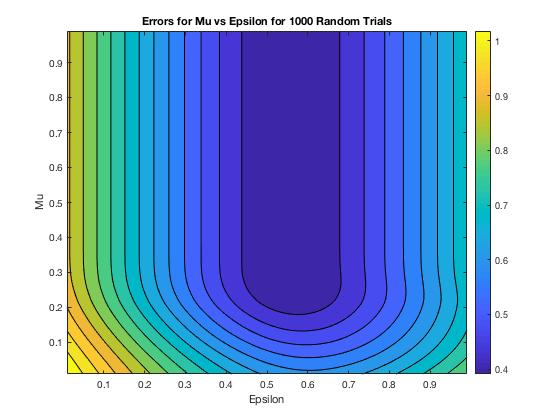
\includegraphics[scale=0.37]{figures/Contour1000WM.jpg}
       \caption{Error contour plot for the Wang Model}
       \label{fig:ContourWang}
   \end{figure} 
    
    %\begin{figure}
    %\centering
    %\begin{minipage}{.5\textwidth}
      %\centering
      %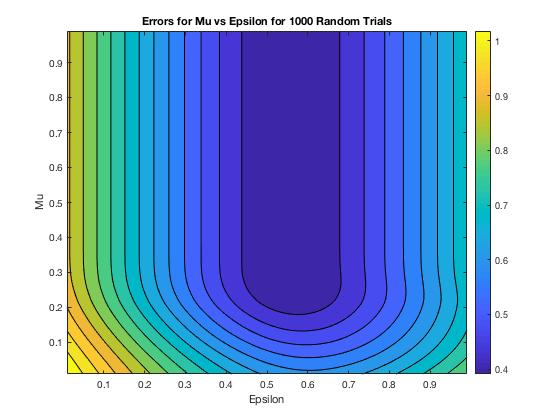
\includegraphics[width=1.1\linewidth]{figures/Contour1000WM.jpg}
    %   \captionof{figure}{Contour Plot of Errors}
      %\label{fig:contourWM}
    %\end{minipage}%
   % \begin{minipage}{.5\textwidth}
      %\centering
    %  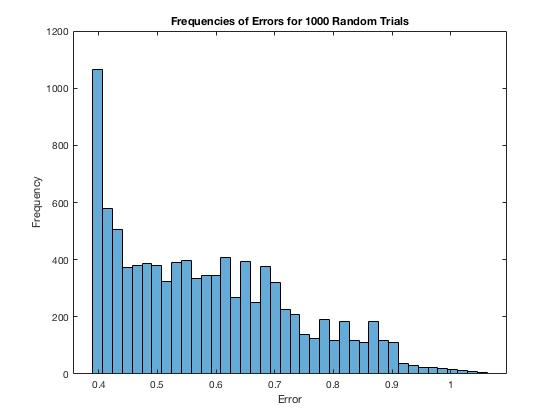
\includegraphics[width=1.1\linewidth]{figures/HistError1000WM.jpg}
    %   \captionof{figure}{Histogram of Errors}
     % \label{fig:histWM}
    %\end{minipage}
    %\end{figure}
    
\end{frame}